\apendice{Documentación técnica de programación}

\section{Introducción}
Este anexo proporciona una documentación detallada sobre la programación del proyecto. Aquí se abordan aspectos cruciales como la estructura de directorios, los pasos para la compilación, instalación y ejecución del proyecto, así como las pruebas del sistema. Este documento está dirigido a desarrolladores que deseen entender y trabajar con el código fuente del proyecto.

\section{Estructura de directorios}
La estructura de directorios del proyecto es fundamental para entender cómo está organizado el código y dónde se encuentran los diferentes componentes. A continuación se muestra una representación visual de la estructura de directorios:

\begin{description}[style=nextline, labelindent=0pt, itemsep=1ex]
    \item[\texttt{TFG-Semi-Supervised-Learning/}:] ruta padre del proyecto
        \begin{description}[style=nextline, labelindent=0pt, itemsep=1ex]
            \item[\texttt{algoritmos/:}] algoritmos de aprendizaje semisupervisado implementados. Cada uno de ellos está programado como una clase, para luego usarlo como un objeto en la aplicación web.
                \begin{description}[style=nextline, labelindent=0pt, itemsep=1ex]
                    \item[\texttt{experimentos:}] contiene notebooks de Jupyter con experimentos y pruebas de los algoritmos de grafos. Puede ser ignorado ya que tiene un propósito de depuración.
                    \item[\texttt{utilidades:}] utilidades que realizan ciertos pasos de la aplicación y de los algoritmos (comunes).
                \end{description}
            \item[\texttt{docs/:}] documentación del proyecto hecha con \LaTeX{}.
                \begin{description}[style=nextline, labelindent=0pt, itemsep=1ex]
                    \item[\texttt{img:}] imágenes utilizadas en la documentación (tanto en la memoria como en la documentación técnica)
                    \item[\texttt{tex:}] archivos \LaTeX{} de la memoria y anexos separados por secciones.
                \end{description}
            \item[\texttt{web/:}] aplicación web de la versión 2.0 del proyecto.
                \begin{description}[style=nextline, labelindent=0pt, itemsep=1ex]
                    \item[\texttt{app/:}] contiene el código fuente de la aplicación web.
                        \begin{description}[style=nextline, labelindent=0pt, itemsep=1ex]
                            \item[\texttt{\_\_init\_\_.py:}] inicializa la aplicación y configura las rutas através del método \texttt{create\_app()}.
                            \item[\texttt{datasets/:}] directorio donde se almacenan los archivos que se usarán en la web.
                                \begin{description}[style=nextline, labelindent=0pt, itemsep=1ex]
                                    \item[\texttt{anonimos/:}] archivos anónimos subidos por los usuarios.
                                    \item[\texttt{registrados/:}] archivos subidos por los usuarios registrados.
                                    \item[\texttt{seleccionar/:}] archivos para probar la aplicación.
                                \end{description}
                            \item[\texttt{static/:}] contiene los archivos estáticos de la aplicación (CSS, JS, imágenes).
                                \begin{description}[style=nextline, labelindent=0pt, itemsep=1ex]
                                    \item[\texttt{css/:}] contiene los estilos CSS de la aplicación. En un único archivo \texttt{style.css}.
                                    \item[\texttt{js/:}] contiene los scripts de JavaScript de la aplicación.
                                        \begin{description}[style=nextline, labelindent=0pt, itemsep=1ex]
                                            \item[\texttt{configuración/:}] scripts de ventana configuración de los algoritmos.
                                            \item[\texttt{usuarios/:}] scripts de ventanas de usuarios.
                                            \item[\texttt{visualización/:}] scripts de ventanas de visualización.
                                        \end{description}
                                    \item[\texttt{json/:}] contiene el archivo de parámetros de configuración de los algoritmos.
                                    \item[\texttt{pseudocodigos/:}] imágenes de los pseudocódigos de los algoritmos (en formato PNG para la web y PDF para el usuario).
                                \end{description}
                            \item[\texttt{runs/:}] directorio donde se almacenan los resultados de las ejecuciones de los algoritmos (en formato JSON).
                            \item[\texttt{templates/:}] contiene las plantillas HTML de la aplicación.
                                \begin{description}[style=nextline, labelindent=0pt, itemsep=1ex]
                                    \item[\texttt{configuracion/:}] plantillas de configuración de los algoritmos.
                                    \item[\texttt{usuarios/:}] plantillas de las ventanas de usuarios.
                                    \item[\texttt{visualizacion/:}] plantillas de las ventanas de visualización.
                                \end{description}
                        \end{description}
                    \item[\texttt{translations/:}]
                        \begin{description}[style=nextline, labelindent=0pt, itemsep=1ex]
                            \item[\texttt{es/:}]
                                \begin{description}[style=nextline, labelindent=0pt, itemsep=1ex]
                                    \item[\texttt{LC\_MESSAGES/:}] contiene los archivos de traducción de la aplicación, el .po será el archivo de traducción y el .mo el archivo compilado.
                                \end{description}
                        \end{description}
                    \item[\texttt{instance:}] contiene la base de datos de la aplicación (SQLite).
                    \item[\texttt{tests:}] contiene el proyecto de pruebas de la aplicación web, hecho con Selenium IDE.
                        \begin{description}[style=nextline, labelindent=0pt, itemsep=1ex]
                            \item[\texttt{ficheros:}] ficheros que se utilizan en las pruebas, uno de error y otro válido.
                        \end{description}
                \end{description}
            \item[\texttt{venv/:}] entorno virtual de Python.
        \end{description}
\end{description}
	
\section{Manual del programador}
En esta sección se comentarán aquellos aspectos que se consideran más relevantes para que un programador pueda entender el \textit{backend} de la aplicación. Para ello, se explicará el proceso típico de adición de un algoritmo, dejando de lado la gestión de usuarios en la que se centra más el trabajo~\cite{TFG:David}. 

La primera fase consiste en la implementación del algoritmo. Hay que tener en cuenta que la versión de Python utilizada es la 3.11 (la más actual hasta el inicio del proyecto). Se debe añadir a la carpeta \texttt{algoritmos} el archivo que contendrá la clase que representa al algoritmo. En el caso de que sea inductivo, los métodos más típicos se deben denominar: \texttt{fit} y \texttt{predict}, para que cuando se lanze desde flask, todo esté automatizado. El método fit, a la vez que va ejecutando el algoritmo, debe ir almacenando en una estructura (preferiblemente \textit{DataFrame}) los datos que se van a representar en la visualización. Para ello el programador debe saber en que lugar y momento del código debe almacenar los datos.

En el otro caso, con los métodos transductivos, existen dos posibles algoritmos, el de la fase de construcción del grafo y el de la fase de inferencia de etiquetas. De nuevo cada uno separado en un archivo que contendrá la definición de una clase. Los algoritmos de construcción de grafos vistos en artículos científicos generalmente reflejan una solución en forma de conjunto de enlaces o en forma de matriz de pesos. Esto no nos interesa en este caso, por lo que se debe buscar la manera de organizar el algoritmo en varias fases (las que se representarán en la web) y devolver los grafos de cada momento o fase. Es decir, lo que devolverá el método de \texttt{construirGrafo} serán varios diccionarios en representación a cada fase del algoritmo. Estos diccionarios deben tener la forma \texttt{\{Número de nodo: [Conjunto de vecinos enlazados], ...\}}. En cuanto a la fase de inferencia, el algoritmo que se quiera implementar, siempre va a necesitar el grafo final construido, para localizar sus enlaces y tenerlos en cuenta. El algoritmo de inferencia depende de cada caso, pero se debe tener un método final que prediga todas las etiquetas de los datos que no estaban etiquetados. En el caso del \textit{Local and Global Consistency} no tiene sentido separar por fases los resultados, ya que puede tener miles de iteraciones variando un mismo resultado esas mil veces, lo que no aporta información valiosa al usuario. En caso de que el algoritmo se pueda dividir en fases, habría que pensar en cómo almacenar los datos para su representación.

Una vez se tienen los algoritmos implementados, es hora de utilizarlos en la web. Para ello, se deben crear los elementos estáticos, como la tarjeta de selección inicial, la opción en el menú de navegación, el pseudocódigo tanto en inglés como en español y un icono representativo. La parte previa a la ejecución de estos nuevos algoritmos será la de configuración. Para ello es importante destacar que existe un archivo llamado \texttt{parametros.json} el cual contiene todos los posibles parámetros de configuración de los clasificadores (en caso de los inductivos) y de los algoritmos (en caso de los transductivos) (ver figura~\ref{fig:anexos/parametros}).

\imagen{anexos/parametros}{Estructura archivo \texttt{parametros.json}}{Contenido del archivo \texttt{parametros.json}}{0.65}

Se debe distinguir en qué clave de entre \textit{Inductive}, \textit{Inference} o \textit{Graphs} se deben incluir los parámetros. Otro detalle importante es que para traducir estos parámetros, como otro recurso diferente a \textit{Babel}, se utiliza un diccionario propio.

Una vez se tienen estos parámetros, se debe seguir el proceso de crear o modificar los métodos:
\begin{itemize}
	\item En \texttt{configuration\_routes}: en el método \texttt{configurar\_algoritmo} se debe crear el formulario correspondiente a cada uno.
	\item  En \texttt{visualization\_routes}: se debe crear un método \texttt{parametros\_algoritmoX}: recogerá los parámetros introducidos en el formulario de configuración y se los pasa a la plantilla HTML.
	\item En la plantilla HTML del algoritmo, se debe crear una llamada al método \texttt{inicializar} o a métodos que hagan lo propio. Este método realiza una petición POST a una ruta no visualizada donde ejecuta los algoritmos. Los parámetros anteriores se pasarán a este nuevo plano y los tendrá en cuenta.
	\item En \texttt{data\_routes}: crear método \texttt{datosAlgoritmoX} el cuál llamará, según su tipo, al método que devuelve toda la información (en formato JSON) de la ejecución. Estos métodos que obtiene los datos instancian la clase del algoritmo y obtienen su resultado. También se encargan de procesar los resultados. Es decir, en los grafos, es necesario sacar la información de: nodos, enlaces, predicciones y mapa de clases; y en los inductivos se deberá obtener: iteraciones, log, estadísticas y mapa de clases.
\end{itemize}

Una vez se tienen los datos procesados, se pueden usar en el javascript y HTML para crear los gráficos y elementos que se crean oportunos.

\section{Compilación, Instalación y Ejecución del Proyecto}

En este apartado se detallan los pasos necesarios para compilar, instalar y ejecutar el proyecto VASS2.

\subsection{Instalación}

Para instalar el proyecto, se deben seguir los siguientes pasos en una terminal del equipo:

\begin{enumerate}
    \item Clonar el repositorio:
    \begin{verbatim}
    git clone https://github.com/msp1015/TFG-Semi-Supervised-Learning
    \end{verbatim}

    \item Navegar al directorio del proyecto:
    \begin{verbatim}
    cd TFG-Semi-Supervised-Learning
    \end{verbatim}

    \item Crear un entorno virtual:
    \begin{verbatim}
    python -m venv ./venv
    \end{verbatim}

    \item Activar el entorno virtual:
    \begin{itemize}
        \item En Windows:
        \begin{verbatim}
        .\venv\Scripts\activate
        \end{verbatim}

        \item En macOS/Linux:
        \begin{verbatim}
        source venv/bin/activate
        \end{verbatim}
    \end{itemize}

    \item Instalar dependencias:
    \begin{verbatim}
    pip install -r requirements.txt
    \end{verbatim}

    \item Creación de directorios necesarios:
    \begin{verbatim}
    cd web/app
    mkdir runs
    \end{verbatim}

    \begin{itemize}
        \item En Windows:
        \begin{verbatim}
        mkdir datasets\anonimos
        mkdir datasets\registrados
        \end{verbatim}

        \item En macOS/Linux:
        \begin{verbatim}
        mkdir datasets/anonimos
        mkdir datasets/registrados
        \end{verbatim}
    \end{itemize}

    \item Compilar traducciones:
    \begin{verbatim}
    pybabel compile -d translations
    \end{verbatim}
\end{enumerate}

\subsection{Uso}

Para ejecutar la aplicación, se deben seguir los siguientes pasos:

\begin{enumerate}
    \item Iniciar la aplicación:
    \begin{verbatim}
    cd ..
    flask run
    \end{verbatim}

    \item Abrir su navegador y navegar a \url{http://localhost:5000} para acceder a la aplicación.

    \item (Opcional) Añadir \texttt{--debug} al final del comando \texttt{flask run} para entrar en modo desarrollo.
\end{enumerate}

\subsection{Despliegue con Gunicorn y Nginx en servidor}

Para desplegar la aplicación en un entorno de producción usando Gunicorn y Nginx en un servidor, siga los siguientes pasos:

\begin{enumerate}
    \item Instalar Gunicorn y Nginx en su máquina de servidor:
    \begin{verbatim}
    sudo apt update
    sudo apt install python3-gunicorn nginx
    \end{verbatim}

    \item Navegar al directorio del proyecto (creado con los pasos vistos en el punto anterior) e iniciar Gunicorn en el puerto 8000:
    \begin{verbatim}
    cd /ruta/a/TFG-Semi-Supervised-Learning/web
    gunicorn -b 0.0.0.0:8000 'app:create_app()'
    \end{verbatim}

    \item Configurar Nginx para servir la aplicación. Abra el archivo de configuración de Nginx:
    \begin{verbatim}
    sudo nano /etc/nginx/sites-available/default
    \end{verbatim}

    \item Añadir la siguiente configuración en el archivo de Nginx:
    \begin{verbatim}
    server {
        listen 80;
        server_name tu_dominio.com;

        location / {
            proxy_pass http://0.0.0.0:8000;
        }
    }
    \end{verbatim}

    \item Guardar y cerrar el archivo, luego reiniciar Nginx:
    \begin{verbatim}
    sudo systemctl restart nginx
    \end{verbatim}

    \item Asegurarse de que Gunicorn y Nginx están ejecutándose correctamente:
    \begin{verbatim}
    sudo systemctl status nginx

    sudo systemctl status gunicorn
    \end{verbatim}
\end{enumerate}

\subsection{Internacionalización con Babel}

Para añadir soporte de internacionalización con Babel, siga los siguientes pasos:

\begin{enumerate}
    \item Extraer los mensajes a traducir:
    \begin{verbatim}
    pybabel extract -F babel.cfg -o messages.pot
    \end{verbatim}

    \item (Opcional) Si utiliza el marcador \texttt{lazy\_gettext} en lugar de \texttt{gettext}, extraer los mensajes de la siguiente manera:
    \begin{verbatim}
    pybabel extract -F babel.cfg -k lazy_gettext -o messages.pot .
    \end{verbatim}

    \item Actualizar el catálogo de traducciones:
    \begin{verbatim}
    pybabel update -i messages.pot -d translations
    \end{verbatim}
	A continuación de este paso se debe traducir el archivo \texttt{messages.po} en la carpeta \texttt{translations}. Además de traducir a mano los textos nuevos, es importante fijarse en aquellos con la etiqueta <<fuzzy>>, ya que pueden generar problemas de traducción y no serán incluidos en la aplicación. Una vez comprobado que estas traducciones estan correctas, se elimina la etiqueta <<fuzzy>>.
    \item Compilar las traducciones:
    \begin{verbatim}
    pybabel compile -d translations
    \end{verbatim}
\end{enumerate}

\section{Pruebas del sistema}
Esta sección del proyecto se centra en las pruebas de la aplicación web para garantizar la calidad y fiabilidad del sistema. Se ha optado por utilizar Selenium IDE debido a sus múltiples ventajas, siendo una heramienta poderosa y fácil de usar e instalar.

En el marco de este proyecto, se ha decidido heredar todos los casos de prueba definidos en el trabajo anterior, garantizando así la continuidad y la cobertura de pruebas ya establecidas. Y se han añadido nuevos casos de prueba para cubrir las nuevas funcionalidades implementadas en la versión 2.0. Se ha necesitado redefinir los anteriores para adaptarlos al nuevo dominio y a una ruta válida de subida de archivos.

En la figura~\ref{fig:anexos/testplan.drawio} se muestra la lista de pruebas que se han hecho en Selenium IDE, organizados en \textit{Test Suites}.

\begin{figure}[H]
	\centering
	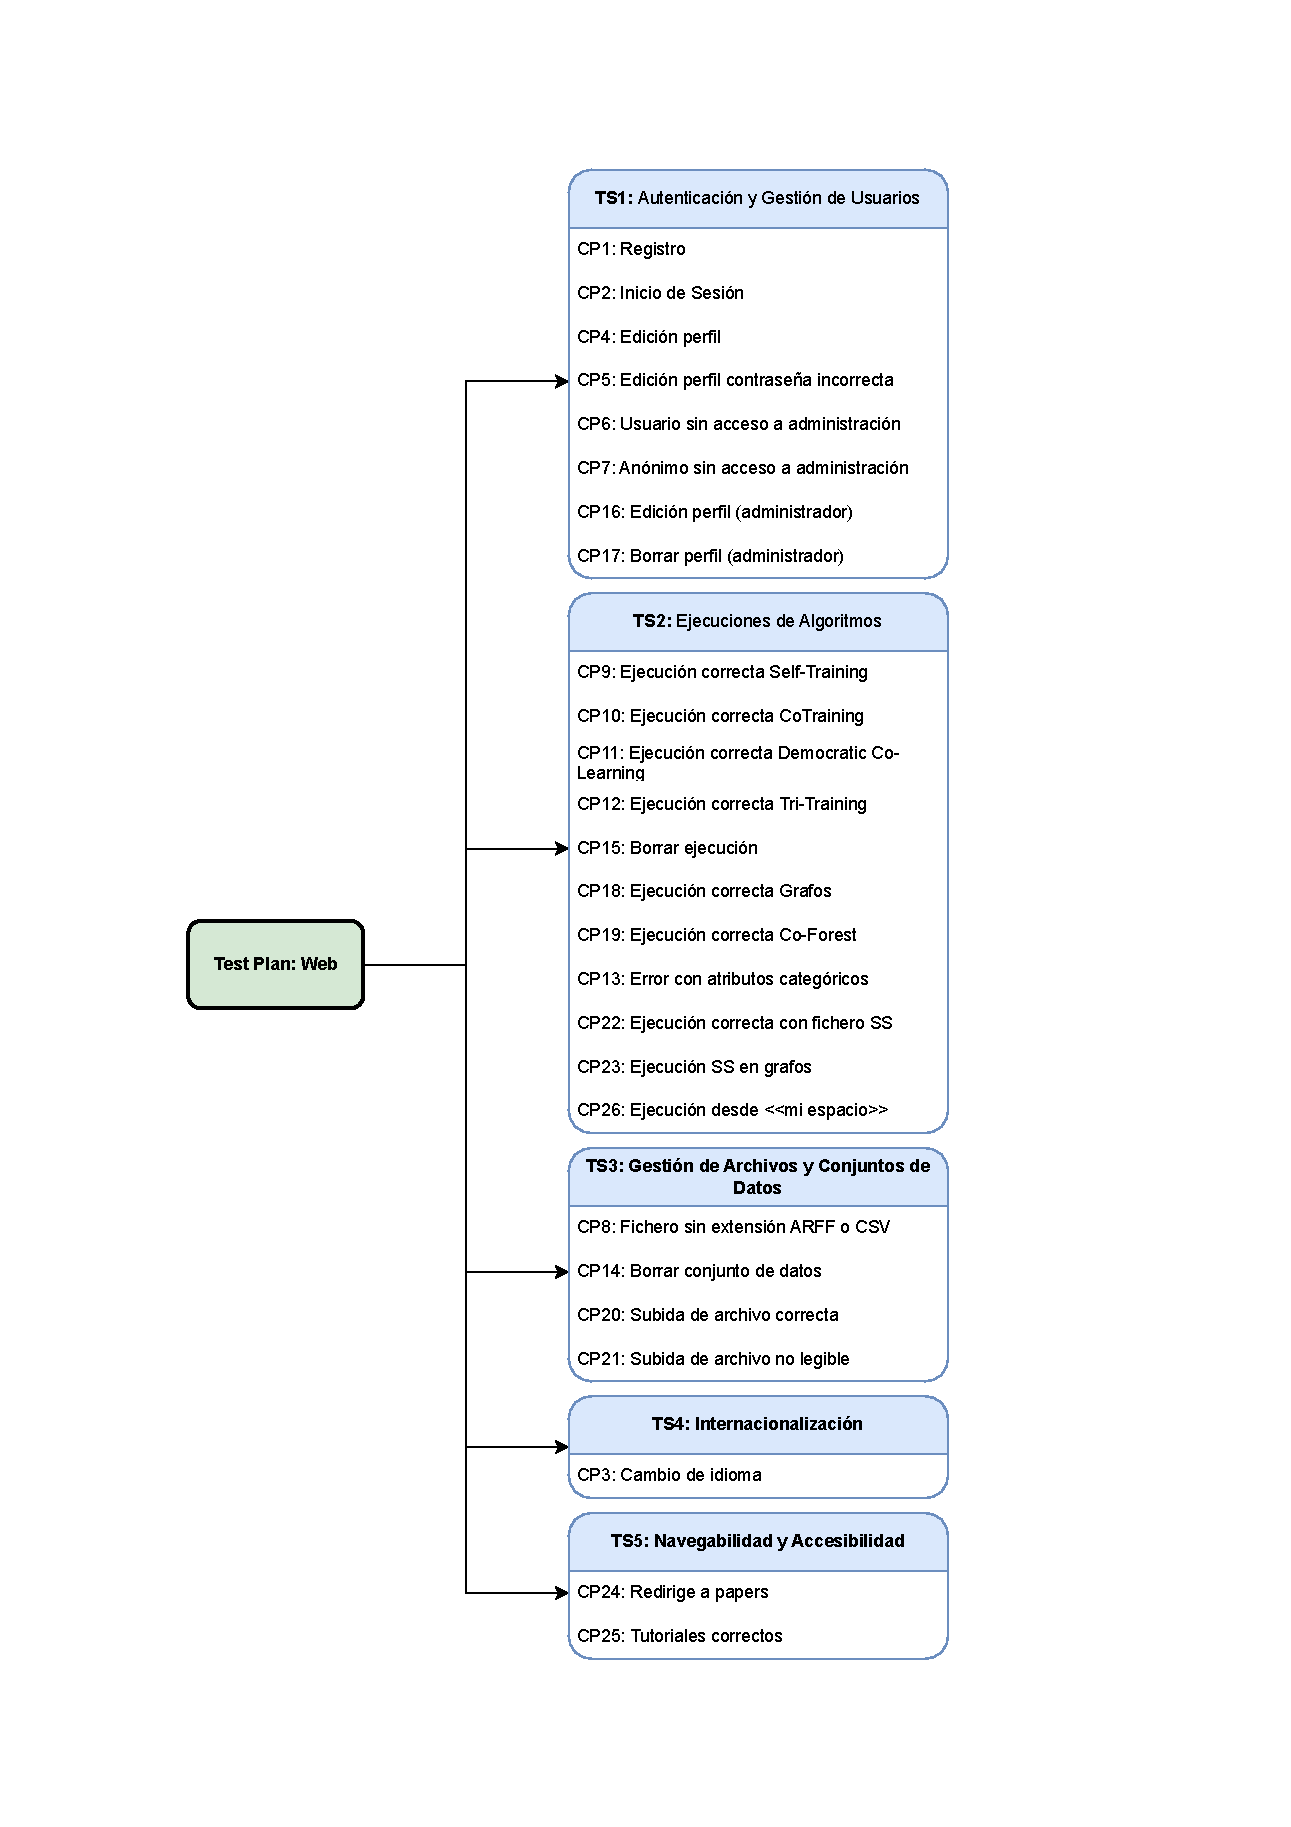
\includegraphics[width=0.80\textwidth]{anexos/testplan.drawio}
	\caption[Test Plan de la Web]{Conjunto de test organizados en Test Suites}\label{fig:anexos/testplan.drawio}
\end{figure}


\begin{table}[ht]
	\centering
	\renewcommand{\arraystretch}{1.5} % Para aumentar el espaciado entre filas
	\begin{tabular}{>{\raggedright\arraybackslash}p{4cm} p{9.5cm}}
    \hline
    \rowcolor{gray!20}
    \textbf{ID} & CP-18\\
    \hline
    \rowcolor{white}
    \textbf{Prioridad} & Alta \\
    \hline
    \rowcolor{gray!20}
    \textbf{Fecha de Ejecución} & 03/07/2024 \\
    \hline
    \rowcolor{white}
    \textbf{Tester} & Mario Sanz Pérez \\
    \hline
    \rowcolor{gray!20}
    \textbf{Descripción} & Ejecución completa de Grafos\\
    \hline
    \rowcolor{white}
    \textbf{Precondiciones} & Sistema en funcionamiento\\
    \hline
    \rowcolor{white}
    \textbf{Datos Utilizados} & \textit{Dataset} proporcionado\\
    \hline
    \rowcolor{gray!20}
    \textbf{Pasos} & \begin{enumerate}
        \item Acceder a vass2.dev/.
        \item Seleccionar la opción de Grafos.
        \item Seleccionar los datos necesarios para la ejecución.
        \item Seleccionar la opción <<Configurar Algoritmo>>.
        \item Comprobar redirección a página de configuración de grafos.
        \item Seleccionar el botón <<Ejecutar>>.
        \item Comprobar redirección a página de resultados comparando el título.
        \item Comprobar existencia de leyenda.
        \item Ejecutar los $n$ pasos hasta la inferencia.
    \end{enumerate}\\
	\hline
    \rowcolor{gray!20}
    \textbf{Resultados esperados} & Ejecución exitosa del algoritmo de Grafos, resultados mostrados correctamente.\\
    \hline
    \rowcolor{white}
    \textbf{Estado} & Exitoso\\
    \hline
\end{tabular}
	\caption[CP18: Ejecución Grafos]{CP18: Ejecución correcta y completa de grafos.}
\end{table}

\begin{table}[ht]
	\centering
	\renewcommand{\arraystretch}{1.5} % Para aumentar el espaciado entre filas
	\begin{tabular}{>{\raggedright\arraybackslash}p{4cm} p{9.5cm}}
    \hline
    \rowcolor{gray!20}
    \textbf{ID} & CP-19\\
    \hline
    \rowcolor{white}
    \textbf{Prioridad} & Alta \\
    \hline
    \rowcolor{gray!20}
    \textbf{Fecha de Ejecución} & 03/07/2024 \\
    \hline
    \rowcolor{white}
    \textbf{Tester} & Mario Sanz Pérez \\
    \hline
    \rowcolor{gray!20}
    \textbf{Descripción} & Ejecución correcta de Co-Forest\\
    \hline
    \rowcolor{white}
    \textbf{Precondiciones} & Sistema en funcionamiento\\
    \hline
    \rowcolor{white}
    \textbf{Datos Utilizados} & \textit{Dataset} para Co-Forest\\
    \hline
    \rowcolor{gray!20}
    \textbf{Pasos} & \begin{enumerate}
        \item Acceder a vass2.dev/.
        \item Seleccionar la opción de Co-Forest.
        \item Seleccionar los datos necesarios para la ejecución.
        \item Seleccionar la opción <<Configurar Algoritmo>>.
        \item Comprobar redirección a página de configuración del Co-Forest.
        \item Seleccionar el botón <<Ejecutar>>.
        \item Comprobar redirección a página de resultados comparando el título.
        \item Comprobar existencia de leyenda.
        \item Comprobar la existencia de estadísticas específicas.
    \end{enumerate}\\
	\hline
    \rowcolor{gray!20}
    \textbf{Resultados esperados} & Ejecución exitosa del algoritmo Co-Forest, resultados mostrados correctamente\\
    \hline
    \rowcolor{white}
    \textbf{Estado} & Exitoso\\
    \hline
\end{tabular}
	\caption[CP19: Ejecución Co-Forest]{CP18: Ejecución correcta y completa de Co-Forest.}
\end{table}

\begin{table}[ht]
	\centering
	\renewcommand{\arraystretch}{1.5} % Para aumentar el espaciado entre filas
	\begin{tabular}{>{\raggedright\arraybackslash}p{4cm} p{9.5cm}}
    \hline
    \rowcolor{gray!20}
    \textbf{ID} & CP-20\\
    \hline
    \rowcolor{white}
    \textbf{Prioridad} & Alta \\
    \hline
    \rowcolor{gray!20}
    \textbf{Fecha de Ejecución} & 03/07/2024 \\
    \hline
    \rowcolor{white}
    \textbf{Tester} & Mario Sanz Pérez \\
    \hline
    \rowcolor{gray!20}
    \textbf{Descripción} & Subida de archivo correcta con usuario registrado\\
    \hline
    \rowcolor{white}
    \textbf{Precondiciones} & Sistema en funcionamiento, archivo válido disponible y usuario en sesión\\
    \hline
    \rowcolor{white}
    \textbf{Datos Utilizados} & Archivo válido en formato ARFF \texttt{iris.arff} y usuario de prueba\\
    \hline
    \rowcolor{gray!20}
    \textbf{Pasos} & \begin{enumerate}
        \item Iniciar sesión en el sistema.
        \item Seleccionar cualquier algoritmo.
        \item Seleccionar la opción para subir un nuevo archivo del equipo.
        \item Confirmar la subida del archivo.
        \item Confirmar la aparición de la tabla con los datos del archivo subido.
        \item Seleccionar el botón <<Mi espacio>>.
        \item Comprobar que existe una entrada en la tabla de datos del archivo subido.
    \end{enumerate}\\
	\hline
    \rowcolor{gray!20}
    \textbf{Resultados esperados} & Archivo subido correctamente, guardado en el sistema y mostrado en forma de tabla\\
    \hline
    \rowcolor{white}
    \textbf{Estado} & Exitoso\\
    \hline
\end{tabular}
	\caption[CP20: Subida de archivo con usuario registrado]{CP20: Subida de archivo con usuario registrado}
\end{table}

\begin{table}[ht]
	\centering
	\renewcommand{\arraystretch}{1.5} % Para aumentar el espaciado entre filas
	\begin{tabular}{>{\raggedright\arraybackslash}p{4cm} p{9.5cm}}
		\hline
		\rowcolor{gray!20}
		\textbf{ID} & CP-21\\
		\hline
		\rowcolor{white}
		\textbf{Prioridad} & Media \\
		\hline
		\rowcolor{gray!20}
		\textbf{Fecha de Ejecución} & 03/07/2024 \\
		\hline
		\rowcolor{white}
		\textbf{Tester} & Mario Sanz Pérez \\
		\hline
		\rowcolor{gray!20}
		\textbf{Descripción} & Subida de archivo no legible sin usuario en sesión\\
		\hline
		\rowcolor{white}
		\textbf{Precondiciones} & Sistema en funcionamiento, archivo no legible disponible\\
		\hline
		\rowcolor{white}
		\textbf{Datos Utilizados} & Archivo no legible \texttt{error.txt}\\
		\hline
		\rowcolor{gray!20}
		\textbf{Pasos} & \begin{enumerate}
			\item Seleccionar cualquier algoritmo.
			\item Seleccionar la opción para subir un nuevo archivo del equipo.
			\item Confirmar la subida del archivo.
			\item Confirmar la aparición de un mensaje de advertencia en lugar de la tabla de datos.
			\item Seleccionar el botón <<Configurar Algoritmo>>.
			\item Comprobar redirección a página de inicio.
			\item Confirmar aparición de mensaje de error.
		\end{enumerate}\\
		\hline
		\rowcolor{gray!20}
		\textbf{Resultados esperados} & El sistema muestra un mensaje de error indicando que el archivo no es legible y redirige a la página de inicio\\
		\hline
		\rowcolor{white}
		\textbf{Estado} & Exitoso\\
		\hline
	\end{tabular}
	\caption[CP21: Subida de archivo ilegible]{CP21: Subida de archivo ilegible}
\end{table}


\begin{table}[ht]
	\centering
	\renewcommand{\arraystretch}{1.5} % Para aumentar el espaciado entre filas
	\begin{tabular}{>{\raggedright\arraybackslash}p{4cm} p{9.5cm}}
    \hline
    \rowcolor{gray!20}
    \textbf{ID} & CP-22\\
    \hline
    \rowcolor{white}
    \textbf{Prioridad} & Alta \\
    \hline
    \rowcolor{gray!20}
    \textbf{Fecha de Ejecución} & 03/07/2024 \\
    \hline
    \rowcolor{white}
    \textbf{Tester} & Mario Sanz Pérez \\
    \hline
    \rowcolor{gray!20}
    \textbf{Descripción} & Ejecución correcta con fichero SS\\
    \hline
    \rowcolor{white}
    \textbf{Precondiciones} & Sistema en funcionamiento, fichero SS disponible\\
    \hline
    \rowcolor{white}
    \textbf{Datos Utilizados} & Fichero \textit{Breast Cancer} semisupervisado \\
    \hline
    \rowcolor{gray!20}
    \textbf{Pasos} & \begin{enumerate}
        \item Acceder a vass2.dev/.
        \item Seleccionar la opción de Co-Forest.
        \item Seleccionar archivo \textit{Breast Cancer} de prueba.
        \item Seleccionar la opción <<Configurar Algoritmo>>.
        \item Comprobar redirección a página de configuración del Co-Forest.
        \item Bajar al mínimo el porcentaje de datos no etiquetados (debe ignorarlo).
        \item Seleccionar el botón <<Ejecutar>>.
        \item Comprobar redirección a página de resultados comparando el título.
        \item Comprobar existencia de leyenda.
        \item Comprobar la existencia de estadísticas específicas.
    \end{enumerate}\\
	\hline
    \rowcolor{gray!20}
    \textbf{Resultados esperados} & Ejecución exitosa del algoritmo con fichero SS, resultados mostrados correctamente\\
    \hline
    \rowcolor{white}
    \textbf{Estado} & Exitoso\\
    \hline
	\end{tabular}
	\caption[CP22: Ejecución con fichero SS]{CP22: Ejecución con fichero semisupervisado}
	
\end{table}

\begin{table}[ht]
	\centering
	\renewcommand{\arraystretch}{1.5} % Para aumentar el espaciado entre filas
	\begin{tabular}{>{\raggedright\arraybackslash}p{4cm} p{9.5cm}}
    \hline
    \rowcolor{gray!20}
    \textbf{ID} & CP-23\\
    \hline
    \rowcolor{white}
    \textbf{Prioridad} & Alta \\
    \hline
    \rowcolor{gray!20}
    \textbf{Fecha de Ejecución} & 03/07/2024 \\
    \hline
    \rowcolor{white}
    \textbf{Tester} & Mario Sanz Pérez \\
    \hline
    \rowcolor{gray!20}
    \textbf{Descripción} & Ejecución SS en grafos\\
    \hline
    \rowcolor{white}
    \textbf{Precondiciones} & Sistema en funcionamiento, datos de grafos disponibles\\
    \hline
    \rowcolor{white}
    \textbf{Datos Utilizados} & Datos de grafos para SS\\
    \hline
    \rowcolor{gray!20}
    \textbf{Pasos} & \begin{enumerate}
		\item Acceder a vass2.dev/.
        \item Seleccionar la opción de Grafos.
        \item Seleccionar archivo \textit{Breast Cancer} de prueba.
        \item Seleccionar la opción <<Configurar Algoritmo>>.
        \item Comprobar redirección a página de configuración del Co-Forest.
        \item Bajar al mínimo el porcentaje de datos no etiquetados (debe ignorarlo).
        \item Seleccionar el botón <<Ejecutar>>.
        \item Comprobar redirección a página de resultados comparando el título.
        \item Comprobar existencia de leyenda.
        \item Pulsar $n$ veces hasta la inferencia.
        \item Seleccionar el botón <<Inferir etiquetas>>.
        \item Comprobar texto de advertencia en resultados (no se puede inferir etiquetas con datos de entrada SS).
    \end{enumerate}\\
	\hline
    \rowcolor{gray!20}
    \textbf{Resultados esperados} & Ejecución exitosa del algoritmo SS con grafos, mensaje de advertencia mostrado correctamente.\\
    \hline
    \rowcolor{white}
    \textbf{Estado} & Exitoso\\
    \hline
\end{tabular}
	\caption[CP23: Ejecución SS en grafos]{CP23: Ejecución de con fichero semisupervisado en grafos}
	
\end{table}

\begin{table}[ht]
	\centering
	\renewcommand{\arraystretch}{1.5} % Para aumentar el espaciado entre filas
	\begin{tabular}{>{\raggedright\arraybackslash}p{4cm} p{9.5cm}}
    \hline
    \rowcolor{gray!20}
    \textbf{ID} & CP-24\\
    \hline
    \rowcolor{white}
    \textbf{Prioridad} & Baja \\
    \hline
    \rowcolor{gray!20}
    \textbf{Fecha de Ejecución} & 03/07/2024 \\
    \hline
    \rowcolor{white}
    \textbf{Tester} & Mario Sanz Pérez \\
    \hline
    \rowcolor{gray!20}
    \textbf{Descripción} & Redirige a artículos científicos\\
    \hline
    \rowcolor{white}
    \textbf{Precondiciones} & Sistema en funcionamiento\\
    \hline
    \rowcolor{white}
    \textbf{Datos Utilizados} & No aplica\\
    \hline
    \rowcolor{gray!20}
    \textbf{Pasos} & \begin{enumerate}
        \item Acceder a vass2.dev/.
        \item Por cada tarjeta de selección: Seleccionar la opción <<Artículo>>.
        \item Verificar la redirección a 6 diferentes pestañas en el navegador.
    \end{enumerate}\\
	\hline
    \rowcolor{gray!20}
    \textbf{Resultados esperados} & El usuario es redirigido correctamente a las 6 páginas científicas.\\
    \hline
    \rowcolor{white}
    \textbf{Estado} & Exitoso\\
    \hline
\end{tabular}
	\caption[CP24: Redirección a artículos]{CP24: Redirección a artículos científicos en la web}
\end{table}

\begin{table}[ht]
	\centering
	\renewcommand{\arraystretch}{1.5} % Para aumentar el espaciado entre filas
	\begin{tabular}{>{\raggedright\arraybackslash}p{4cm} p{9.5cm}}
    \hline
    \rowcolor{gray!20}
    \textbf{ID} & CP-25\\
    \hline
    \rowcolor{white}
    \textbf{Prioridad} & Media \\
    \hline
    \rowcolor{gray!20}
    \textbf{Fecha de Ejecución} & 03/07/2024 \\
    \hline
    \rowcolor{white}
    \textbf{Tester} & Mario Sanz Pérez \\
    \hline
    \rowcolor{gray!20}
    \textbf{Descripción} & Tutoriales correctos en todas las páginas\\
    \hline
    \rowcolor{white}
    \textbf{Precondiciones} & Sistema en funcionamiento, botón de <<tutorial>> existe\\
    \hline
    \rowcolor{white}
    \textbf{Datos Utilizados} & No aplica\\
    \hline
    \rowcolor{gray!20}
    \textbf{Pasos} & \begin{enumerate}
        \item Acceder a vass2.dev/.
        \item Seleccionar la opción <<Tutorial>>.
        \item Comprobar texto de cada paso del turorial de inicio.
        \item Seleccionar un algoritmo, ejemplo: Co-Forest.
        \item Seleccionar la opción <<Tutorial>>.
        \item Comprobar texto de cada paso del tutorial de subida de archivo.
        \item Seleccionar la opción <<Configurar Algoritmo>>.
        \item Seleccionar la opción <<Tutorial>>.
        \item Comprobar texto de cada paso del tutorial de configuración de algoritmo.
        \item Seleccionar la opción <<Ejecutar>>.
        \item Seleccionar la opción <<Tutorial>>.
        \item Comprobar texto de cada paso del tutorial de resultados.
    \end{enumerate}\\
	\hline
    \rowcolor{gray!20}
    \textbf{Resultados esperados} & Los tutoriales se muestran correctamente y son accesibles para el usuario (tanto anónimo como registrado)\\
    \hline
    \rowcolor{white}
    \textbf{Estado} & Exitoso\\
    \hline
\end{tabular}
	\caption[CP25: Ejecución de tutoriales]{CP25: Ejecución de tutoriales en todas las ventanas.}
\end{table}

\begin{table}[ht]
	\centering
	\renewcommand{\arraystretch}{1.5} % Para aumentar el espaciado entre filas
	\begin{tabular}{>{\raggedright\arraybackslash}p{4cm} p{9.5cm}}
    \hline
    \rowcolor{gray!20}
    \textbf{ID} & CP-26\\
    \hline
    \rowcolor{white}
    \textbf{Prioridad} & Media \\
    \hline
    \rowcolor{gray!20}
    \textbf{Fecha de Ejecución} & 03/07/2024 \\
    \hline
    \rowcolor{white}
    \textbf{Tester} & Mario Sanz Pérez \\
    \hline
    \rowcolor{gray!20}
    \textbf{Descripción} & Ejecución desde <<mi espacio>>\\
    \hline
    \rowcolor{white}
    \textbf{Precondiciones} & Usuario autenticado, acceso a <<mi espacio>>, ejecución previa almacenada en base de datos\\
    \hline
    \rowcolor{white}
    \textbf{Datos Utilizados} & Usuario de Prueba, ejecución almacenada con fichero X\\
    \hline
    \rowcolor{gray!20}
    \textbf{Pasos} & \begin{enumerate}
        \item Acceder a <<mi espacio>> desde la interfaz de usuario.
        \item Seleccionar el algoritmo deseado en la tabla de historial.
        \item Comprobar redirección a página de resultados comparando el título.
        \item Comprobar existencia de leyenda.
        \item Comprobar la existencia de estadísticas específicas.
    \end{enumerate}\\
	\hline
    \rowcolor{gray!20}
    \textbf{Resultados esperados} & Ejecución exitosa del algoritmo desde <<mi espacio>>, resultados mostrados correctamente\\
    \hline
    \rowcolor{white}
    \textbf{Estado} & Exitoso\\
    \hline
    \end{tabular}
	\caption[CP26: Ejecución desde cuenta de usuario]{CP26: Ejecución desde cuenta de usuario registrado.}
\end{table}

